% ответы на вопросы
\newpage
\section*{Ответы на вопросы}
\addcontentsline{toc}{section}{\tocsecindent{Ответы на вопросы}}
\begin{enumerate}
    \item\Large{Как синтаксически представляется программа на Lisp, и как она хранится в памяти?}\\
    	Lisp формы представления программы и обрабатываемых ею данных одинаковы. И то и другое представляется списочной структурой имеющей одинаковую форму. Поэтому программы могут обрабатывать и преобразовывать другие программы или сами себя. 
    \item\Large{Как трактуются элементы списка?}\\
    	Если это  не стоит блокировка вычисления(quote $\equiv$ '), то первый элемент трактуется как имя функции, остальные — как аргументы.
    \item\Large{Порядок реализации программы?}\\
    	\underline{Программа работает в цикле:}
		\begin{enumerate}
			\item Ожидает ввода S-выражение
			\item Передает введенное S-выражение функции eval
			\item Выводит полученный результат
		\end{enumerate}
	\begin{minipage}[t]{1.0\textwidth}
	\raggedleft
		\centering\raisebox{\dimexpr \topskip-\height}{%
		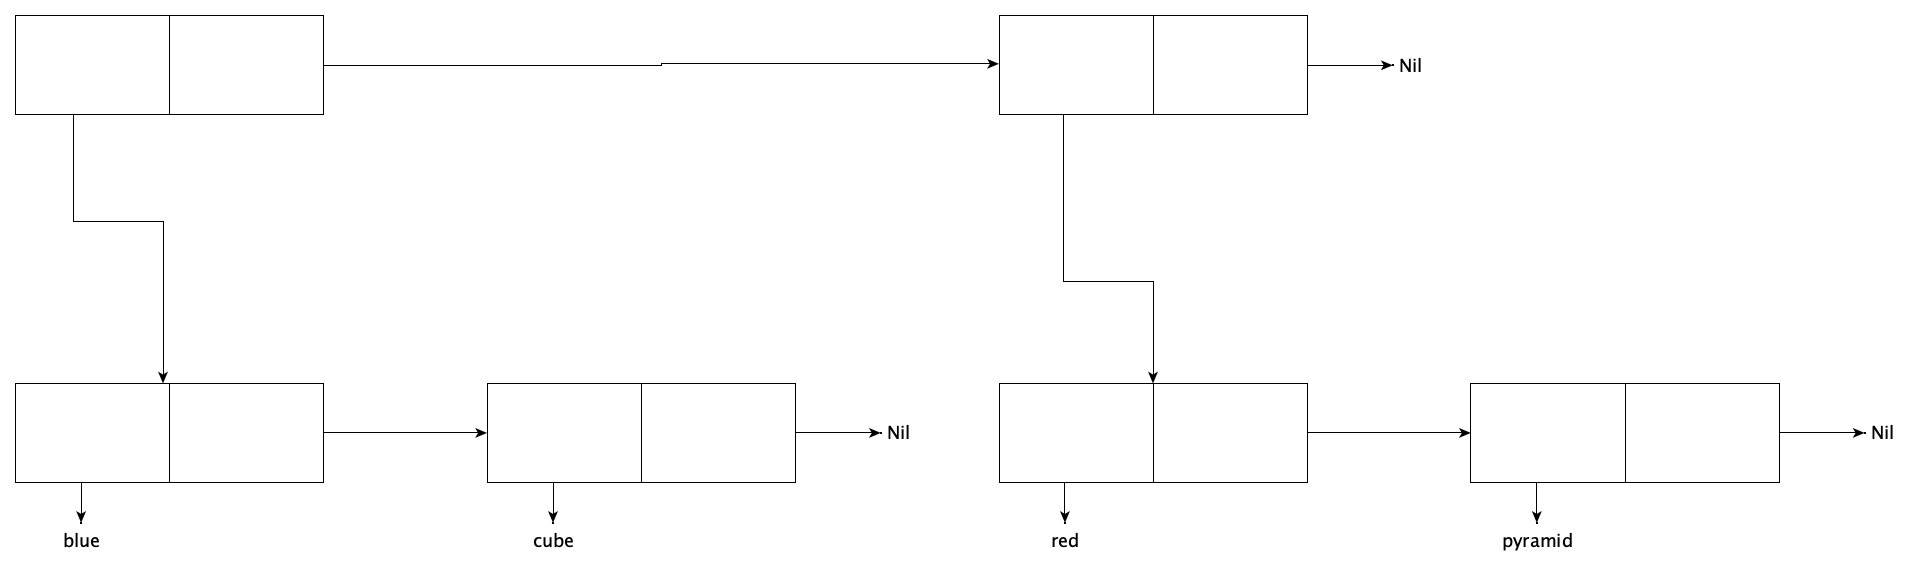
\includegraphics[width=\textwidth]{1.png}}
		\captionof{figure}{eval S-выражение}
		\label{fig2}
	\end{minipage}\hfill
\end{enumerate}

% ответ
%\\